\documentclass[11pt,a4paper]{article}

\usepackage{fontspec}
\usepackage{xeCJK}
\setCJKmainfont{FandolSong-Regular.otf}[BoldFont=FandolSong-Bold.otf,
                                        ItalicFont=FandolKai-Regular.otf]
\setCJKsansfont{FandolHei-Regular.otf}[BoldFont=FandolHei-Bold.otf]
\setCJKmonofont{FandolFang-Regular.otf}
\usepackage[margin=1in]{geometry}
\usepackage{amsmath,amssymb,amsthm}
\usepackage{graphicx}
\usepackage{booktabs,longtable,array,calc}
\usepackage{tikz}
\usetikzlibrary{positioning,arrows.meta}
\usepackage{microtype}
\usepackage{xcolor}
\usepackage[hidelinks]{hyperref}
\usepackage{caption}
\usepackage{float}
\usepackage{etoolbox}
\hypersetup{pdftitle={The Mathematical Limits of AI Reliability: Inevitable Failure under Strong Causality},pdfauthor={Zhizhi Liao (廖至智)}}
\AtBeginEnvironment{longtable}{\small}
\setlength{\tabcolsep}{4pt}
\renewcommand{\arraystretch}{1.12}
\captionsetup{font=small,labelfont=bf,skip=6pt}
\graphicspath{{./}}
\setlength{\emergencystretch}{3em}
\setcounter{secnumdepth}{0}
\setcounter{tocdepth}{0}
\providecommand{\tightlist}{\setlength{\itemsep}{0pt}\setlength{\parskip}{0pt}}
\newcounter{none}
\AtBeginEnvironment{thebibliography}{\footnotesize\setlength{\itemsep}{0pt}\linespread{0.97}\selectfont}

\title{\bfseries The Mathematical Limits of AI Reliability\\[2pt]
\large Inevitable Failure under Strong Causality}
\author{Zhizhi Liao (廖至智) \\
Independent Researcher \\
\texttt{liaozhizhi@foxmail.com}}
\date{November 2026}

\begin{document}
\maketitle

\begin{abstract}
\noindent
\label{abstract}

Systems that report on their own success fail characteristically: they claim a
scope they did not deliver in the act of stopping. We study this failure in
\textbf{strong causal environments}, where claim and fact are separated by a physical
transition the model can trigger but not edit; same-origin evaluation cannot
detect it.

We separate what is arithmetic from what is a claim about the world. When evaluator
and policy read one observation and share one prior, the verdict is a measurable
function of that pair, so \(I(V;T\mid O,\Pi)=0\) follows from how the evaluator is
wired rather than from any property of evaluation; we state it as an identity and
do not argue from it. The statement with content is what remains once the prior is
removed from the conditioning set: on the part of the distribution where the record
does not cover the prior's support, the verdict cannot lower the error of a
decision that already sees the record by more than \(\eta(\mathrm{cov}(o))\), with
\(\eta(0)=0\). In-distribution, where the prior is informative, \(\eta\) is large and
the bound is silent --- and there the verdict can and does correlate with the truth.
The bound bites on the tail, and the tail is where the tasks are worth automating.
No retraining of the evaluator moves it. Three things do: coverage, a record rich
enough to determine the outcome, and an added channel to the world.

We measured an evaluator with zero mutual information with the truth---this is a
calculation, not an estimate. Across ten trajectories, four failing, the untrained
base model answered \texttt{PASS} ten times. A constant carries no bits, so the
information is zero by the definition of entropy, with no asymptotics and no
independence assumption.

Two further results locate the consequence: a per-step false-completion rate bounds
the probability of at least one undetected failure along a conjunctive chain,
exponentially only under step independence, which we refute by counterexample; and
a finite trust chain whose transitions cannot read the truth has no repair
mechanism from inside, and under a separate erosion assumption (H2) --- an empirical
assumption, measurable and not universal --- its healthy states are transient, so
failure is not corrected but outlived. An external physical witness is the only
intervention that adds a channel rather than improving one; its value is bounded by
what the witness itself knows.
\end{abstract}

\vspace{1.2em}

\section{1. Introduction}\label{introduction}

There is a class of tasks where ``did the model succeed?'' has an answer
independent of the model's opinion, and where being wrong is costly. We call
these \textbf{strong causal environments}: claim and fact are separated by a physical
transition the model can trigger but cannot edit. Code either runs or
raises\textasciitilde{}\cite{jimenez2023swebench}; a braking distance is either shorter than the
obstacle or it is not. What matters
there is not fluency or likelihood, but whether the world moved and whether the
system noticed.

The failure we study is not hallucination in the ordinary sense. A model that
invents a citation is wrong about a text. A model that reports \texttt{PASS} on a build
that did not compile is wrong about the world, and the wrongness is invisible
from inside the loop that produced it. We call this a \textbf{false completion}: the
system claims a scope it did not deliver, in the same act by which it decides to
stop. Its danger is independent of capability, because it terminates the process
that could have found the error. A system that keeps failing is annoying; one
that declares success and halts is a liability, since no further evidence is
collected.

The empirical situation is worse than the vocabulary suggests. Before any
training, the base model behind a preference-tuning experiment was asked to
adjudicate four trajectories that had demonstrably failed; it returned \texttt{PASS} on
all four. On six succeeding trajectories it also returned \texttt{PASS}. Across ten
items the evaluator was not merely optimistic, it was \textbf{constant}. We do not
treat that as an anecdote: it identifies which hypothesis below is satisfied in
practice, and in §2.8 it collapses one asymptotic statement into an identity. A
constant carries exactly zero bits, so an evaluator that always says \texttt{PASS} has
mutual information zero with the truth --- not approximately, not in the limit,
exactly.

\subsection{1.1 Why the existing remedies do not reach the problem}\label{why-the-existing-remedies-do-not-reach-the-problem}

\textbf{Text-only preference optimisation.} Direct preference
optimisation\textasciitilde{}\cite{rafailov2023dpo} reshapes a policy from pairs of preferred and
dispreferred outputs. When those pairs come
from the same prior being corrected --- the normal case, since annotator, judge and
policy share a training distribution --- the optimisation moves the \emph{distribution
of the output} without changing the \emph{relation between output and world}. Its
objective is a tool-layer report: a margin, a loss curve, accuracy on held-out
pairs. A report can be optimised to perfection while the behaviour it certifies
is untouched. Above, the objective saturated while the grounded response was
produced on zero prompts. §3.1 formalises this: an intervention on the
evaluator's parameters is not an intervention on the truth, so no setting of them
creates information the channel does not carry.

\textbf{Variance-based monitoring.} A second family watches dispersion of outputs,
confidence or rewards and flags instability. This cannot work, for an elementary
reason: variance is translation invariant, \(\mathrm{Var}(X+c)=\mathrm{Var}(X)\).
A monitor measuring spread is blind by construction to a \emph{constant} bias, and the
measured failure mode is exactly a constant. The worse the deception, the more
stable it looks. Dispersion measures inconsistency, not incorrectness --- noise on
one side, a fixed offset that averaging never removes on the other.

Both families lack a channel to the world that is not the model's own report.
That lack is our object.

\subsection{1.2 What we prove}\label{what-we-prove}

\textbf{An identity, and then the theorem (Theorem 2).} Under same-origin evaluation ---
evaluator and policy read the same observation and share a prior --- the verdict is a
measurable function of \((O,\Pi)\), so \(I(V;T\mid O,\Pi)=0\). We state that as
Proposition 7 and do not call it a result: for an evaluator wired this way it is
automatic, and it is not the kind of statement a measurement can refute. The result
of the section is Theorem 2, which drops the prior from the conditioning set. Under
a coverage condition on the prior --- (A2.2\('\)), an empirical assumption we label as
such --- the error of any decision that reads the verdict is within
\(\eta(\mathrm{cov}(o))\) of the error of a decision that reads only the record.
Inside the prior's coverage \(\eta\) is large and the bound says nothing; on the tail
\(\eta\to0\) and the verdict's contribution vanishes. The bound is therefore about a
channel where the channel matters, which is narrower than ``the verdict carries no
information'' and is the only version we can defend.

\textbf{An accumulation law (Theorem 1).} If each step produces a false completion
with probability at least \(\epsilon\), the probability of at least one undetected
false completion over an \(n\)-step chain is at least \(1-(1-\epsilon)^n\) --- under
step independence. We also prove the independence-free bound, and give the
counterexample showing the exponential rate is unavailable without it; this is
the weakest of the three, and we say so in the text.

\textbf{An absorption theorem (Theorem 3).} Model trust in the system's own verdicts
as a finite Markov chain with a bankruptcy state. If transitions do not take the
truth as an input, no repair conditional on failure can exist; under a separate
erosion assumption (H2), healthy states are then transient and absorption is almost
sure. Neither half is proved here from first principles, and we say which is which:
the chain algebra is textbook, the erosion condition is an empirical assumption, and
the lemma in between is the one that says why the truth cannot be an input --- the
same-origin assumption again.

Together they give one conclusion with a precise scope: an external physical
witness --- a channel to the world that is neither the model's report nor a
read-out of its prior --- is the only operation that \emph{adds} a channel to the decision.
We formalise it (Definition 4), give it a value (Corollary 3), and show that value
belongs to the witness alone, so improving the evaluator cannot substitute for
acquiring one.

\subsection{1.3 What we do not claim}\label{what-we-do-not-claim}

We do not claim reliability is impossible. We claim it is bounded, and identify
the bound and its escape. A witness is necessary for escaping it, not sufficient
for reliability.

Two things do move the bound, and naming them costs us the slogan that nothing
does. \textbf{Coverage} moves it: (A2.2) is a statement about which part of the
distribution the record occupies, so a prior that has been trained on the tail is
not uninformative on the tail, and \(\eta(\mathrm{cov}(o))\) is written in the form
it is written so that this can be measured rather than argued. \textbf{A record that
determines the outcome} moves it too, and §3.2 measures the move: adding execution
hashes and exit codes to the record raised forced-choice accuracy from \(0.60\) to
\(0.80\), because a truth reading had entered \(O\). What does \emph{not} move the bound is
the evaluator. No retraining of \(\phi\) changes \(I(V;T\mid O,\Pi)\), and none changes
\(\eta\); scaling the evaluator acts inside the conditioning set. So the correct
statement is narrower than ``scale cannot help'': scale helps exactly to the extent
that it changes coverage or enriches the record, and the experiments that would
separate those from a genuine improvement of judgement are not in this paper.

And we present no benchmark: every number here appears once, in §3, to identify
which hypothesis the measured system satisfies.

A note on the title. \emph{Inevitable} is used throughout in its measure-theoretic
sense --- almost sure, with respect to the measure named in the theorem --- and the
extent is always written. Where a statement is a positive probability rather than
a probability of one, it appears as \(\epsilon\) or as a bound, never as rhetoric.
The word carries no weight that the equations do not carry.

\section{2. Definitions, the Causal Graph, and Three Theorems}\label{definitions-the-causal-graph-and-three-theorems}

\subsection{2.0 Notation and the four-valued verdict}\label{notation-and-the-four-valued-verdict}

Random variables are written in upper case, their values in lower case, and
\(p_X\) denotes the law of \(X\). All entropies and mutual informations are in nats
unless stated otherwise. For a joint law, \(H(X\mid Y)\) is the conditional
entropy and \(I(X;Y\mid Z)\) the conditional mutual information; the data
processing inequality is written \(X\to Y\to Z\Rightarrow I(X;Z)\le I(X;Y)\)
\cite{cover2006elements}.

The verdict \(V\) is \textbf{four-valued}, not Boolean:
\begin{equation}
\mathcal V=\{\texttt{PASS},\ \texttt{FAIL},\ \texttt{INVALID},\ \texttt{NOT\_RUN}\}.
\tag{2.0.1}
\end{equation}
This matters for what follows. The distinction between \texttt{FAIL} and \texttt{INVALID} is not
decoration: \texttt{FAIL} asserts that a scope existed and was not delivered, whereas
\texttt{INVALID} asserts that the question had no referent. Collapsing the two would
make the bound below look tighter than it is. We keep all four.

{\def\LTcaptype{none} % do not increment counter
\begin{longtable}[]{@{}
  >{\raggedright\arraybackslash}p{(\linewidth - 4\tabcolsep) * \real{0.3333}}
  >{\raggedright\arraybackslash}p{(\linewidth - 4\tabcolsep) * \real{0.3333}}
  >{\raggedright\arraybackslash}p{(\linewidth - 4\tabcolsep) * \real{0.3333}}@{}}
\toprule\noalign{}
\begin{minipage}[b]{\linewidth}\raggedright
symbol
\end{minipage} & \begin{minipage}[b]{\linewidth}\raggedright
meaning
\end{minipage} & \begin{minipage}[b]{\linewidth}\raggedright
type
\end{minipage} \\
\midrule\noalign{}
\endhead
\bottomrule\noalign{}
\endlastfoot
\(E=(\mathcal S,\mathcal A,P,s_0,v)\) & strong causal environment & Definition 1 \\
\(\mathcal S,\ \mathcal A\) & state and action spaces & standard Borel \\
\(P\) & transition kernel \((\mathcal S\times\mathcal A)\times\mathcal B(\mathcal S)\to[0,1]\) & Markov kernel \\
\(v\) & truth function \(\mathcal S\times\mathcal A\to\{0,1\}\) & measurable \\
\(Z_t\) & step truth \(v(s_t,a_t)\) & \(\{0,1\}\) \\
\(T=T_n=\bigwedge_{t=1}^{n}Z_t\) & chain truth & \(\{0,1\}\) \\
\(\pi_\theta\) & policy & conditional law on \(\mathcal A\) \\
\(V_\phi\) & same-origin evaluator & \(\mathcal V\) \\
\(O\) & observation channel & random element \\
\(\Pi\) & shared prior & random element \\
\(W\) & independent witness & random element \\
\(\epsilon\) & false-\texttt{PASS} rate under failure & \((0,1]\) \\
\(U\) & exogenous factor of the environment & random element \\
\(X_k\) & trust-chain state & \(\{0,\dots,K\}\) \\
\(\eta(\cdot)\) & prior-coverage slack & \([0,1]\)-valued \\
\(\Delta_{\mathrm{wit}}\) & value of a witness & \(\mathbb R_{\ge0}\) \\
\end{longtable}
}

Two conventions that are used throughout and are not re-stated each time:
\(O\) denotes the whole record available to the model at decision time, not a
single frame; and conditioning on \(O\) always means conditioning on the
\(\sigma\)-algebra \(\sigma(O)\), so that ``given \(O\)'' is a statement about
information, not about a particular value.

\begin{center}\rule{0.5\linewidth}{0.5pt}\end{center}

\subsection{2.1 Definition 1 --- the strong causal environment}\label{definition-1-the-strong-causal-environment}

\textbf{Definition 1.} A strong causal environment is a tuple
\[
E=\big(\mathcal S,\ \mathcal A,\ P,\ s_0,\ v\big),
\qquad
P:\mathcal S\times\mathcal A\to\Delta(\mathcal S),
\qquad
v:\mathcal S\times\mathcal A\to\{0,1\},
\]
with \((\mathcal S,\mathcal B(\mathcal S))\) a standard Borel space, \(\mathcal A\)
Borel, \(s_0\in\mathcal S\), \(P\) a Markov kernel and \(v\) measurable. A run of
length \(n\) is a sequence \((s_t,a_t)_{t\ge1}\) with \(s_1=s_0\),
\(a_t\sim\pi_\theta(\cdot\mid s_t)\), \(s_{t+1}\sim P(\cdot\mid s_t,a_t)\).

\textbf{Definition 1.1 (step truth).} For \(t\ge1\),
\[
Z_t:=v(s_t,a_t)\in\{0,1\}.
\]

\textbf{Axiom A1 (non-writability).} The truth is a function of the realised state and
action and of nothing else:
\begin{equation}
Z_t\ \ \text{is}\ \ \sigma(s_t,a_t)\text{-measurable}.
\tag{A1}
\end{equation}

A1 is weaker than the phrase ``the environment cannot be tampered with''. That
phrase is an engineering claim about sandboxes and permissions; A1 is a
measurable-structure claim that can be used in a proof. It has an immediate and
useful consequence: because \(Z_t\) is \(\sigma(s_t,a_t)\)-measurable, it is
conditionally independent of \emph{every} other random element given \((s_t,a_t)\),
including the model parameters. Writing \(\theta\) for those parameters,
\begin{equation}
Z_t\ \perp\!\!\!\perp\ \theta\ \mid\ (s_t,a_t).
\tag{A1.1}
\end{equation}

\textbf{Definition 1.2 (task chain).} A task chain of length \(n\) succeeds iff every
step succeeds:
\begin{equation}
T_n:=\bigwedge_{t=1}^{n}Z_t,
\qquad
\{\text{success}\}=\{T_n=1\}.
\tag{2.1.1}
\end{equation}

The conjunction is the substance of ``strong causality'': one broken link breaks the
chain. Nothing below requires the steps to be identically distributed, and
nothing requires them to be independent --- that distinction becomes the whole
content of §2.7.

\textbf{Proposition 1 (when the prior-independence axiom is free).} Let
\(O^{\mathrm{full}}:=(s_{0:t},a_{0:t})\) be the complete record up to \(t\). Then
\(T_n\) is \(\sigma(O^{\mathrm{full}})\)-measurable, hence
\begin{equation}
I\big(T_n;\Pi\ \big|\ O^{\mathrm{full}}\big)=0
\qquad\text{for every random element }\Pi .
\tag{2.1.2}
\end{equation}
\emph{Proof.} By Definition 1.2 and A1, \(T_n\) is a measurable function of
\((s_{0:n},a_{0:n})=O^{\mathrm{full}}\), so \(H(T_n\mid O^{\mathrm{full}})=0\) and the
mutual information vanishes. \(\square\)

Proposition 1 locates the difficulty precisely. When the record is complete,
the assumption that the prior is uninformative about the truth (A2.2 below) costs
nothing --- it is a theorem. The assumption has content only for a \textbf{lossy} record,
which is the realistic case: the model does not observe the full state, and the
gap is filled in by its prior. This is exactly the regime in which the prior can
help, and the next section states when it does not.

\begin{center}\rule{0.5\linewidth}{0.5pt}\end{center}

\subsection{2.2 Definition 2 --- same-origin evaluation}\label{definition-2-same-origin-evaluation}

\textbf{Definition 2.} An evaluator \(V_\phi\) is \emph{same-origin} with a policy
\(\pi_\theta\) if there exist a random element \(\Pi\) and measurable maps \(f,g\) such
that
\begin{equation}
\theta=f(\Pi),\qquad \phi=g(\Pi),
\tag{D2.a}
\end{equation}
and if, in addition, the evaluator reads no information channel that the policy
does not read:
\begin{equation}
T\ \perp\!\!\!\perp\ V\ \mid\ (O,\Pi).
\tag{D2.1}
\end{equation}

Clause (D2.a) says the two functions are two read-outs of one prior; (D2.1) says
they share one channel. Together they are the formal content of ``there is no
independent physical witness''. (D2.1) is not an assumption about the \emph{strength} of
the evaluator. An arbitrarily large, well-trained evaluator satisfies it as long
as everything it has ever seen arrived through \(O\) and its own prior.

\textbf{Proposition 2 ((D2.1) is a d-separation statement).} (D2.1) holds iff \(T\) and
\(V\) are d-separated by \((O,\Pi)\) in the graph of §2.5. In that graph the only
path from \(T\) to \(V\) is \(T\leftarrow U\to O\to V\), and conditioning on \(O\) blocks
it.

\textbf{Axiom A2.2 (prior uninformative on the tail).} The distinction the axiom
formalises is the epistemic one: uncertainty that further evidence can remove,
as opposed to noise that it cannot\textasciitilde{}\cite{hullermeier2021aleatoric}. On the
low-coverage event
\[
\mathrm{Low}_\kappa:=\big\{o:\ \mathrm{cov}(o)\le\kappa\big\},
\]
where \(\mathrm{cov}(o)\in[0,1]\) is the \(\Pi\)-mass of the region of the prior's
support consistent with the record \(o\), the prior adds nothing to the record:
\begin{equation}
T\ \perp\!\!\!\perp\ \Pi\ \mid\ O=o
\qquad\text{for}\quad o\in\mathrm{Low}_\kappa .
\tag{A2.2}
\end{equation}

\textbf{The quantitative form.} In practice (A2.2) is not exact, and stating it as
though it were would be the single easiest way to have this paper dismissed. We
therefore use the following relaxation throughout, and give the exact version only
as the \(\eta\equiv0\) special case:
\begin{equation}
\mathrm{TV}\Big(p_{T\mid O=o,\,\Pi}\ ,\ p_{T\mid O=o}\Big)\ \le\ \eta\big(\mathrm{cov}(o)\big),
\qquad \eta(0)=0,
\tag{A2.2'}
\end{equation}
with \(\eta\) non-decreasing. A2.2\('\) says: the amount by which the prior can improve
on the record is bounded by how much of the prior's support the record occupies.
On the tail, \(\mathrm{cov}(o)\to0\) and the slack vanishes with it.

\begin{quote}
\textbf{Why this is the right hypothesis, and not a convenient one.} Strong-causal
tasks are precisely those where the prior has little to say: the braking
distance on ice at an unusual load, the interaction between two drugs that were
never co-prescribed, the build that fails only under an uncommon allocator.
These are not adversarial constructions; they are the reason the tasks are
worth automating. In-distribution, A2.2 can fail --- the prior genuinely knows
something --- and there the bound below simply does not bind. The claim of this
paper is therefore not ``evaluation is always uninformative'' but \textbf{``evaluation is
uninformative exactly where the stakes are''}, which is a narrower and, we
think, more uncomfortable statement.
\end{quote}

\begin{center}\rule{0.5\linewidth}{0.5pt}\end{center}

\subsection{2.3 Definition 3 --- the optimistic prior, and the measurement that locates it}\label{definition-3-the-optimistic-prior-and-the-measurement-that-locates-it}

\textbf{Axiom A3 (optimistic prior).} There is \(\epsilon>0\) such that
\begin{equation}
\Pr\big[V_\phi=\texttt{PASS}\ \big|\ Z=0\big]\ \ge\ \epsilon .
\tag{A3.1}
\end{equation}

\textbf{Measured instance.} In the companion study, the untrained base model was asked
to adjudicate ten trajectories: four that had demonstrably failed and six that had
succeeded. It answered \texttt{PASS} on all ten. We use this in exactly one way, and it
is worth being explicit about what that way is: it tells us that (A3.1) holds with
\(\epsilon=1\), and it tells us that in the measured regime \(V\) is a \textbf{constant}.
The second fact is much stronger than the first, and §2.8 turns it into an
identity rather than a bound.

\textbf{Proposition 3 (dispersion monitors are structurally blind).} Let
\(M=\mathrm{Var}(V_\phi)\) be any monitor that scores the evaluator by the
dispersion of its output. Then
\begin{equation}
M(V_\phi+c)=M(V_\phi)\quad\text{for all }c,
\qquad\text{and in particular}\qquad
V_\phi\equiv\texttt{PASS}\ \Rightarrow\ M=0 .
\tag{2.3.1}
\end{equation}
Consequently, on the set of constant evaluators, \(M\) assigns the same value to
one that always says \texttt{PASS} and one that always says \texttt{FAIL}: a false completion on
every failure and a false completion on none are indistinguishable to it. No
threshold on a variance-based monitor separates them.

\emph{Proof.} \(\mathrm{Var}(X+c)=\mathrm{Var}(X)\) and \(\mathrm{Var}(c)=0\). \(\square\)

Proposition 3 is the formal counterpart of §1.1's second paragraph, and it is
why the empirical observation is not a coincidence: the failure mode with the
largest bias is also the one with the smallest dispersion.

\begin{center}\rule{0.5\linewidth}{0.5pt}\end{center}

\subsection{2.4 Definition 4 --- the independent witness}\label{definition-4-the-independent-witness}

\textbf{Definition 4.} A random element \(W\) is an \emph{independent witness} for the truth
\(T\) relative to the record \(O\) if
\begin{equation}
T\ \not\perp\!\!\!\perp\ W\ \mid\ O
\qquad\text{and}\qquad
W\ \perp\!\!\!\perp\ \Pi\ \mid\ (T,O).
\tag{D4.1}
\end{equation}

The first clause says \(W\) carries information about the truth that \(O\) does not
already carry. The second says \(W\) is not a read-out of the prior. Both are
needed, and the second is the one that is usually skipped.

\textbf{Proposition 4 (the second clause is not implied by the first).} There is a
witness satisfying the first clause of (D4.1) and violating the second, whose
information gain is zero.

\emph{Proof.} Take \(W:=V_\phi\) itself --- the evaluator offered as its own witness. The
first clause of (D4.1) then holds whenever the evaluator is at all correlated with
the truth. The second fails, because \(W\) is a measurable function of \((O,\Pi)\).
And the value is zero: \(I(W;T\mid O,V)=I(V;T\mid O,V)=0\), since \(V\) is determined
by \((O,V)\). The same computation applies to any second evaluator
\(W=V_{\phi'}\) with \(\phi'=h(\Pi)\) for which \(T\perp\Pi\mid O\) holds. This is the
``witness that is only another opinion''. \(\square\)

Proposition 4 is the reason the definition is written with two clauses rather
than one, and it also supplies the operational test below: a candidate witness is
worth exactly its conditional mutual information given the record and the
verdict, and that quantity can be estimated on held-out trajectories.

\textbf{The escape criterion.} For a candidate witness \(W\), define
\begin{equation}
\mathrm{Esc}(W):=\Big[\,I\big(W;T\ \big|\ O,V\big)>0\,\Big].
\tag{2.4.1}
\end{equation}
\(\mathrm{Esc}(W)\) is the property that matters; it is a computable functional of
the joint law, not a stipulation about how \(W\) was produced.

\begin{center}\rule{0.5\linewidth}{0.5pt}\end{center}

\subsection{2.5 The causal graph, d-separation, and what an intervention can do}\label{the-causal-graph-d-separation-and-what-an-intervention-can-do}

The assumptions of §2.1--2.4 are summarised by Figure 1. Nodes are random
elements; the absence of an edge is a substantive claim.

\begin{figure}[H]
\centering
% The causal graph of Section 2.5. The edge that is missing is the theorem.
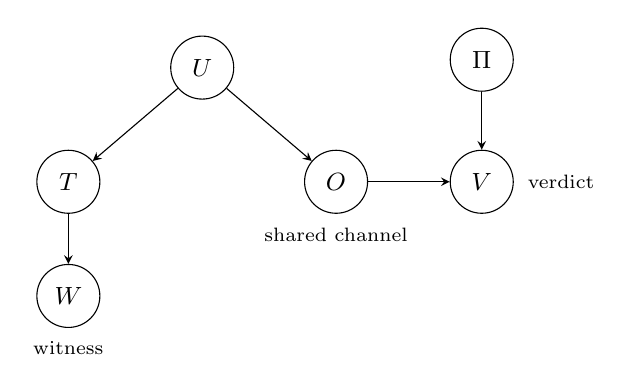
\begin{tikzpicture}[
  >=stealth,
  state/.style={circle,draw,inner sep=1.5pt,minimum size=8mm,font=\small},
  note/.style={draw=none,inner sep=2pt,font=\scriptsize}
]
  \node[state] (U)  at (0.00, 0.00) {$U$};
  \node[state] (T)  at (-1.70,-1.45) {$T$};
  \node[state] (O)  at (1.70,-1.45) {$O$};
  \node[state] (V)  at (3.55,-1.45) {$V$};
  \node[state] (Pi) at (3.55, 0.10) {$\Pi$};
  \node[state] (W)  at (-1.70,-2.90) {$W$};

  \draw[->] (U) -- (T);
  \draw[->] (U) -- (O);
  \draw[->] (O) -- (V);
  \draw[->] (Pi) -- (V);
  \draw[->] (T) -- (W);

  \node[note, below=1mm of O] {shared channel};
  \node[note, right=1mm of V] {verdict};
  \node[note, below=1mm of W] {witness};
\end{tikzpicture}

\caption{The causal graph of the hypotheses. $U$ is the environment's
exogenous factor and the common cause of the truth $T$ and the record $O$;
that edge is what makes the record informative. $O\to V$ and $\Pi\to V$
are the two inputs of a same-origin evaluator. The edge that is missing,
$T\to V$, is the hypothesis (D2.1), i.e. the factorisation identity of Proposition 7. The arrow
$T\to W$ is a witness: an arrow out of the truth that bypasses $O$.}
\label{fig:dag}
\end{figure}


Reading the graph:

\begin{itemize}
\tightlist
\item
  \(U\) is the environment's exogenous factor. It is the common cause of the truth
  \(T\) and the record \(O\): this edge is what makes the record informative at all.
\item
  \(O\to V\) and \(\Pi\to V\) are the two inputs of a same-origin evaluator. There is
  \textbf{no} edge \(T\to V\) --- that missing edge \emph{is} the hypothesis (D2.1).
\item
  \(T\to W\) is the witness. A witness is, by construction, an arrow out of the
  truth that bypasses \(O\).
\end{itemize}

The same graph in TikZ (the source of the figure; MathJax does not
render it):

\textbf{Proposition 5 (the bound, by d-separation).} In the graph above, \(T\) and \(V\)
are d-separated by \(\{O,\Pi\}\). Hence (D2.1) holds, hence
\begin{equation}
I\big(V;T\ \big|\ O,\Pi\big)=0 .
\tag{2.5.1}
\end{equation}

\emph{Proof.} The only path from \(T\) to \(V\) is \(T\leftarrow U\to O\to V\). It is a chain
through \(O\), and \(O\) is in the conditioning set, so the path is blocked. The edge
\(T\to W\) leads nowhere, since \(W\) is not an ancestor of \(V\). Every path is
blocked, so the d-separation holds; by the vertex separation theorem of directed
graphs\textasciitilde{}\cite{pearl2009causality}, d-separation implies conditional independence,
which is (D2.1).
\(\square\)

Proposition 5 is the reason the paper is organised around a graph rather than
around a bare information inequality. A claim of the form ``\(I(V;T)=0\)'' is
false in general --- an evaluator can and often does correlate with the truth --- and
a referee is entitled to reject it with a single counterexample. A claim of the
form ``\(T\) is d-separated from \(V\) by \((O,\Pi)\)'' is a statement about a mechanism,
it can be checked edge by edge, and it can be broken in exactly one way.

\textbf{What an intervention can and cannot do.} Let \(do(\phi:=\phi')\) denote
replacing the evaluator's parameters. Since \(\phi\) is not an ancestor of \(T\) in
the graph,
\begin{equation}
\Pr\big[T\ \big|\ do(\phi:=\phi')\big]=\Pr[T]
\qquad\text{for every }\ \phi',
\tag{2.5.2}
\end{equation}
so no retraining of the evaluator moves the truth. More to the point, the \emph{bound}
is invariant as well:
\begin{equation}
I\big(V_{\phi'};T\ \big|\ O,\Pi\big)=0
\qquad\text{for every }\ \phi',
\tag{2.5.3}
\end{equation}
because the missing edge \(T\to V\) is a property of the graph, not of the
parameters. Equation (2.5.3) is the formal statement of ``preference tuning cannot
repair this'', and §3.1 elaborates it. Conversely, \(do(V:=\texttt{PASS})\) --- lying
harder --- does not change \(T\) either; you cannot improve the world by misreporting
it, and you cannot learn about it by misreporting it.

The one intervention that changes (2.5.1) is structural: add the edge \(T\to W\),
and let the decision read \(W\). This is what (D4.1) encodes, and it is why the
witness is not a better evaluator but a second channel.

\begin{center}\rule{0.5\linewidth}{0.5pt}\end{center}

\subsection{2.6 The assumption ledger (Table A0)}\label{the-assumption-ledger-table-a0}

Every assumption the argument uses, with its kind. The kind matters more than the
label, because it decides what a reader is entitled to do with a theorem that
cites it. We use three kinds and no others.

\begin{itemize}
\tightlist
\item
  \textbf{S (structural).} Holds because of how the object is defined or wired. Not an
  empirical claim, and not something data can overturn. (D2.1) is of this kind: an
  evaluator that reads only \((O,\Pi)\) is a measurable function of \((O,\Pi)\).
\item
  \textbf{M (modelling).} A choice about the model, which a different model could make
  differently. Asserted, not measured, and defended by the fact that the results
  are stated conditionally on it.
\item
  \textbf{E (empirical).} A claim about a distribution in the world. Measurable, in
  principle refutable by a measurement, and \textbf{not} universal. A theorem that cites
  an E-assumption is a conditional statement about systems in which that
  measurement comes out favourably; it is not a law.
\end{itemize}

{\def\LTcaptype{none} % do not increment counter
\begin{longtable}[]{@{}
  >{\raggedright\arraybackslash}p{(\linewidth - 8\tabcolsep) * \real{0.2000}}
  >{\raggedright\arraybackslash}p{(\linewidth - 8\tabcolsep) * \real{0.2000}}
  >{\raggedright\arraybackslash}p{(\linewidth - 8\tabcolsep) * \real{0.2000}}
  >{\raggedright\arraybackslash}p{(\linewidth - 8\tabcolsep) * \real{0.2000}}
  >{\raggedright\arraybackslash}p{(\linewidth - 8\tabcolsep) * \real{0.2000}}@{}}
\toprule\noalign{}
\begin{minipage}[b]{\linewidth}\raggedright
label
\end{minipage} & \begin{minipage}[b]{\linewidth}\raggedright
kind
\end{minipage} & \begin{minipage}[b]{\linewidth}\raggedright
statement
\end{minipage} & \begin{minipage}[b]{\linewidth}\raggedright
load-bearing for
\end{minipage} & \begin{minipage}[b]{\linewidth}\raggedright
if removed
\end{minipage} \\
\midrule\noalign{}
\endhead
\bottomrule\noalign{}
\endlastfoot
A1 & S & \(Z_t=v(s_t,a_t)\) & A1.1; Proposition 1 & environment can be edited; the problem changes \\
A2 (D2.1) & S & \(T\perp V\mid(O,\Pi)\) & Proposition 7, Lemma 1 & the record would not exhaust the verdict \\
A2.2 & \textbf{E} & \(T\perp\Pi\mid O\) on low-coverage \(O\) & Corollary 2 & only the quantitative form, Theorem 2, survives \\
A2.2\('\) & \textbf{E} & TV slack \(\eta(\mathrm{cov})\) & Theorem 2 & the bound is vacuous, not false; only \(\eta\equiv0\) survives \\
A3 & M & \(\Pr[\texttt{PASS}\mid Z=0]\ge\epsilon>0\) & Theorem 1 & no accumulation to bound \\
A5 & M & step independence & the \emph{rate} in Theorem 1 & linear bound only; see Proposition 6 \\
H1 & S & \(\lvert\mathcal X\rvert<\infty\) & Theorem 3 & the finite-state argument \\
H2 & \textbf{E} & erosion: every transient state has positive hazard into \(0\) & Theorem 3, Theorem 3\('\) & no almost-sure absorption; the chain may be irreducible \\
L1(i)--(ii) & M & update has no \(T\) input; \(X_k\) summarises the record & Lemma 1 & marginal transition may inherit \(T\) \\
\end{longtable}
}

\textbf{The two E-entries are the ones a reader should press on, and we say why.} A2.2
and H2 are not axioms and we do not number them as such. Each is a claim about a
distribution that a measurement could refute:

\begin{itemize}
\tightlist
\item
  A2.2 fails if, on records where \(\mathrm{cov}(o)\le\kappa\), the prior still
  improves on the record --- that is, if \(\eta(\mathrm{cov}(o))\) turns out to be
  bounded away from zero on the tail. §4.4 states this as the paper's first
  falsifier, and \(0.60\to0.80\) in §3.2 is a partial instance of the prior improving
  once the record is enriched, which is why A2.2\('\) and not A2.2 is the form we use.
\item
  H2 fails if trust can persist on a set of states from which bankruptcy is
  unreachable. A system that never loses trust because it never notices anything
  wrong satisfies Lemma 1 and violates H2, and Theorem 3 does not apply to it. We
  state this in §2.9 rather than hide it, and we do not claim that H2 is necessary
  for the phenomenon --- only that it is the condition under which the chain argument
  gives absorption.
\end{itemize}

Two further entries deserve comment. A2.2\('\) is how we keep the argument alive when
A2.2 is attacked, at the price of a slack term that is itself measurable. A5 is the
weakest assumption in the paper and is discussed in §2.7, where it is also refuted
in the direction that matters. A5 is labelled M rather than E because the mechanism
it denies --- one prior, one blind spot, positively correlated errors --- is a
modelling claim about how the deployment is built, and §2.7 exhibits what happens
when it is false.

\begin{center}\rule{0.5\linewidth}{0.5pt}\end{center}

\subsection{2.7 Theorem 1 --- the accumulation law}\label{theorem-1-the-accumulation-law}

\textbf{Definition (false completion).} For \(t\ge1\),
\begin{equation}
A_t:=\big\{V_\phi(s_t,a_t)=\texttt{PASS}\big\}\cap\{Z_t=0\}.
\tag{2.7.1}
\end{equation}

\textbf{Axiom A5 (step independence).} The events \(A_1,\dots,A_n\) are mutually
independent. A5 is used only for the rate in (2.7.3); it is not needed for
(2.7.2), (2.7.4) or (2.7.6), and §2.7 shows that it fails in the regime of
interest.

\textbf{Theorem 1.} The following hold, in decreasing strength of hypothesis.

\textbf{(1.1) No assumption (union bound).}
\begin{equation}
\Pr\Big[\bigcup_{t=1}^{n}A_t\Big]\ \le\ \sum_{t=1}^{n}\Pr[A_t]\ \le\ n\,\epsilon .
\tag{2.7.2}
\end{equation}

\textbf{(1.2) Independent steps (geometric decay).} If \(A_1,\dots,A_n\) are independent
and \(\Pr[A_t]\ge\epsilon\) for all \(t\), then
\begin{equation}
\Pr\Big[\bigcap_{t=1}^{n}A_t^{\mathsf c}\Big]
=\prod_{t=1}^{n}\big(1-\Pr[A_t]\big)\ \le\ (1-\epsilon)^{n}.
\tag{2.7.3}
\end{equation}

\textbf{(1.3) Exact criterion for the infinite product.} Let \(\epsilon_t:=\Pr[A_t]\).
\begin{equation}
\prod_{t=1}^{\infty}(1-\epsilon_t)=0
\qquad\Longleftrightarrow\qquad
\sum_{t=1}^{\infty}\epsilon_t=\infty .
\tag{2.7.4}
\end{equation}

\textbf{(1.4) Self-termination.} Let \(\nu:=\inf\{t: V_\phi=\texttt{PASS}\}\) be the
policy's own stopping rule. Then under independence
\begin{equation}
\Pr[\nu\le n]=1-\prod_{t=1}^{n}(1-\epsilon_t),
\qquad\text{which tends to }1\text{ whenever }\textstyle\sum_t\epsilon_t=\infty .
\tag{2.7.5}
\end{equation}

\textbf{(1.5) Partial completion (a deviation bound, not a reliability bound).} Let
\(S_n=\frac1n\sum_{t\le n}Z_t\) and \(\hat S_n=\frac1n\sum_{t\le n}\mathbf{1}[V_\phi=\texttt{PASS}]\).
Then
\begin{equation}
\mathbb E\big|\hat S_n-S_n\big|
\ \le\ \underbrace{\Pr[V=\texttt{PASS},\,Z=0]}_{\le\,\epsilon}
+\underbrace{\Pr[V\ne\texttt{PASS},\,Z=1]}_{=:\ \delta_{\mathrm{miss}}}
\ \le\ \epsilon+\delta_{\mathrm{miss}},
\tag{2.7.6}
\end{equation}
independently of \(n\).

\emph{Proofs.} (1.1) is subadditivity plus (A3.1). (1.2) is the product formula for
independent events, plus \(1-q_t\le1-\epsilon\) when \(q_t\ge\epsilon\). For (1.3),
take logarithms: \(\log\prod(1-\epsilon_t)=\sum\log(1-\epsilon_t)\), and use
\(\log(1-x)\le-x\) together with \(\log(1-x)\ge-2x\) for \(0<x\le\frac12\); the tail of
the sum decides convergence, so the product vanishes iff \(\sum\epsilon_t\)
diverges. (1.4) is \(\{\nu\le n\}=\bigcup_{t\le n}A_t\) with (1.2). For (1.5),
triangle inequality on the difference of empirical means, and note that
\(|\mathbf{1}[V=\texttt{PASS}]-Z|\le\mathbf{1}[V=\texttt{PASS},Z=0]+\mathbf{1}[V\ne\texttt{PASS},Z=1]\).
\(\square\)

\textbf{The assumption that does the work, and why it fails.} The rate in (2.7.3) is
entirely due to independence. In the systems we care about, independence is
false in a specific direction: one prior, one blind spot, so errors are positively
correlated. The following counterexample shows that positive correlation makes
the \emph{no-false-completion} probability larger, not smaller.

\textbf{Proposition 6 (the exponential rate is not available without A5).} Fix
\(\epsilon\in(0,1)\) and consider a chain that fails at every step, \(Z_t=0\) for all
\(t\le n\) --- a task that cannot be done. Let the evaluator commit once per episode:
draw \(U\sim\mathrm{Bern}(\epsilon)\) and set \(V_\phi=\texttt{PASS}\) on \(\{U=1\}\)
and \(V_\phi=\texttt{FAIL}\) on \(\{U=0\}\), for every \(t\). Then A3 holds with equality,
\(\Pr[A_t]=\epsilon\) for every \(t\), and
\begin{equation}
\Pr\Big[\bigcap_{t=1}^{n}A_t^{\mathsf c}\Big]=1-\epsilon
\qquad\text{whereas}\qquad
(1-\epsilon)^{n}\downarrow0 .
\tag{2.7.7}
\end{equation}
\emph{Proof.} \(A_t=\{U=1\}\) for every \(t\), so all \(A_t\) coincide and the intersection is
\(\{U=0\}\). \(\square\)

This is the smallest possible deviation from the hypotheses of (2.7.3): the marginals
\(\Pr[A_t]=\epsilon\) are exactly as required, and A3 holds with equality. Only the
dependence is different, and it makes the clean-run probability \emph{independent of
\(n\)}. The counterexample therefore isolates A5 and nothing else. The interpretation
is not exotic: an evaluator that forms one opinion per episode and repeats it is
the normal case, not the pathological one.

Proposition 6 is not a technicality; it is a correction to how Theorem 1 may be
read. \textbf{Theorem 1 must not be read as ``errors accumulate''.} What accumulates,
under independence, is the chance of at least one false completion; under positive
correlation, that chance can be smaller while each individual report is just as
wrong. The quantity that degrades with \(n\) regardless of correlation is the
\emph{discrepancy between report and truth}, and that is the object of §2.8 --- of Theorem 2
in particular, because the discrepancy is what the decision error is made of.

Theorem 1's honest role is therefore narrower than its statement suggests, and we
prefer to say so: it is the arithmetic of a per-step false-positive rate under an
assumption that real systems violate. Its useful content is (1.5): on
average-scored tasks the report can be off by at most \(\epsilon+\delta_{\mathrm{miss}}\)
no matter how long the chain, which is the formal reason a high single-step
accuracy coexists with long-chain failure and a benchmark that looks fine.

\begin{center}\rule{0.5\linewidth}{0.5pt}\end{center}

\subsection{2.8 What a verdict carries}\label{what-a-verdict-carries}

\textbf{The order of this section is deliberate.} It states two propositions, four
corollaries, and then Theorem 2 at the end. The first proposition is what (D2.1)
yields immediately, and it is a statement about measurable functions rather than
about evaluation; the second is a claim about one measured artefact. Theorem 2 is
what remains when we stop conditioning on the prior, which is the situation any
deployment is actually in. It comes last because it is the statement that degrades
gracefully rather than failing outright when the tail assumption is weakened.

\textbf{Proposition 7 (the factorisation identity).} Under (D2.1), for every environment
of Definition 1 and every evaluator satisfying Definition 2,
\begin{equation}
\boxed{\ I\big(V;T\ \big|\ O,\Pi\big)=0\ }
\tag{2.8.1}
\end{equation}
with probability one, i.e.~the conditional law factorises
\(p_{V,T\mid O,\Pi}=p_{V\mid O,\Pi}\,p_{T\mid O,\Pi}\).

\emph{Proof.} (D2.1) \emph{is} the factorisation; the mutual information of two random
elements that are conditionally independent given \(Z\) is zero, since
\(I(V;T\mid Z)=D_{\mathrm{KL}}\big(p_{V,T\mid Z}\,\|\,p_{V\mid Z}p_{T\mid Z}\big)\)
and the argument of the logarithm is \(1\) almost surely. \(\square\)

\textbf{This is not the paper's contribution, and we no longer present it as one.} The
proof is one line because the conclusion is contained in the hypothesis, and the
hypothesis is close to automatic. An evaluator is a map from what it can read to a
verdict. If what it can read is \((O,\Pi)\), then \(V\) is \(\sigma(O,\Pi)\)-measurable,
and for a measurable function of \((O,\Pi)\) the conditional independence (D2.1) is
not a claim about the evaluator's quality but a consequence of how it is wired.
Three apparent openings close the same way. A deterministic evaluator satisfies
(D2.1) by measurability. A randomised evaluator that draws independent noise
satisfies it because independent noise carries nothing about \(T\). An evaluator that
reads some further channel is excluded by the second clause of Definition 2, which
says in words that it reads nothing the policy does not read.

Equation (2.8.1) is therefore true, and it is the reason no amount of work on the
evaluator can help, but it distinguishes no deployment from any other and no
measurement can refute it. We keep it because every statement below is phrased
relative to it --- it fixes what ``no information beyond the record'' means --- and
because it locates the content of the paper by exclusion: the content is not in the
quality of the evaluator, and it is not in (2.8.1).

Where the content is has two halves, and they must be kept apart. Off the
low-coverage part of the distribution, the record and the prior may determine the
truth; the verdict may then correlate with the truth through the record, and
\(I(V;T)\) may be large. Nothing in (2.8.1) says otherwise, and any reading of it as
``\(I(V;T)=0\)'' is simply false. On the low-coverage part --- the tail, where
strong-causal tasks live --- the prior has nothing to add to the record, and there
the verdict's \emph{marginal} contribution can be shown to vanish. The first half is
Corollary 1; the exact form of the second half is Corollary 2; and the form that
survives an inexact tail assumption is Theorem 2, at the end of this section.

\textbf{Corollary 1 (data-processing upper bound, and what it does not say).}
\begin{equation}
I(V;T)\ \le\ I\big(V;(O,\Pi)\big)\ \le\ \min\big\{H(V),\,H(O,\Pi)\big\}.
\tag{2.8.2}
\end{equation}
This is an upper bound, not a vanishing quantity. \(I(V;T)\) can be strictly
positive, because \(O\) carries information about \(T\); the record is informative
even when the verdict is not. Any claim of the form ``\(I(V;T)\to0\)'' is false in
general and is not made here.

Inside the support of the prior this is the normal case and not a defect: the
verdict inherits whatever the record knows about the truth, and \(I(V;T)\) can be
large. §3.2 measures the inherited part \emph{growing} when the record is enriched ---
forced-choice accuracy rises from \(0.60\) to \(0.80\) once execution hashes and exit
codes enter \(O\) --- and every point of that gain appears on the right-hand side of
(2.8.2), arriving through the record. What the verdict does not do is add to
\((O,\Pi)\). Corollary 1 is therefore the first half of the paper's claim: it says
the verdict can be informative, and it also says that all of its information is
borrowed.

\textbf{Corollary 2 (posterior invariance; the exact tail case).} (A2.2) is asserted
only on \(\mathrm{Low}_\kappa\), so read this corollary conditioned on a record
\(o\in\mathrm{Low}_\kappa\): if \(T\perp\Pi\mid O=o\) at that record, then for every
\(y\in\mathcal V\),
\begin{equation}
\Pr\big[T=1\ \big|\ V=y,\,O\big]=\Pr\big[T=1\ \big|\ O\big],
\qquad
\ell(y):=\log\frac{\Pr[V=y\mid T=1,O]}{\Pr[V=y\mid T=0,O]}=0 .
\tag{2.8.3}
\end{equation}
Consequently, for any decision rule \(\hat T\),
\begin{equation}
\inf_{\hat T(\cdot)}\Pr\big[\hat T(V,O)\ne T\big]
\ =\
\inf_{\hat T'(\cdot)}\Pr\big[\hat T'(O)\ne T\big].
\tag{2.8.4}
\end{equation}
The verdict cannot improve on the record: it is not that reading \(V\) makes the
error larger, but that it cannot make it smaller. The likelihood ratio the verdict
contributes is exactly \(1\) throughout.

\emph{Proof.} From (D2.1) and \(T\perp\Pi\mid O\) one obtains \(T\perp(V,\Pi)\mid O\) by
the contraction property of conditional independence; the conditional law of \(T\)
given \((V,O)\) therefore does not depend on \(y\), giving (2.8.3). For (2.8.4): the
direction \(\le\) is immediate, since a rule that ignores \(V\) is a rule that uses
\((V,O)\); the reverse direction follows from (2.8.3): a rule that uses \(V\) has the
same risk as the randomised rule that draws \(V\sim p_{V\mid O}\) and then ignores
it, and randomisation cannot beat the optimal deterministic rule on \(O\). Both
directions together give equality. \(\square\)

\textbf{What Corollary 2 says on the tail, in one sentence.} Where (A2.2) holds exactly,
the verdict is informationally dead: conditionally on the record,
\(I(V;T\mid O)=0\), and the Bayes error of any decision equals that of a decision
that never reads \(V\). This is the exact half of the paper's claim, and it is exact
rather than asymptotic for a reason worth stating: \(V\) is a function of \((O,\Pi)\),
and the hypothesis removes \(\Pi\) from the conditioning set, so what is left of \(V\)
is a function of \(O\) alone and adds nothing to \(O\). Corollary 2 is therefore the
statement ``on the tail the verdict contributes zero'', and it fails only if (A2.2)
fails.

\textbf{Proposition 8 (the measured evaluator).} If \(V\equiv y_0\) almost surely, then
for \textbf{every} joint law of \((T,O)\),
\begin{equation}
I(V;T)=0,
\qquad
I(V;T\mid O)=0,
\qquad
\Pr[T=1\mid V]=\Pr[T=1].
\tag{2.8.5}
\end{equation}
\emph{Proof.} A constant is measurable with respect to the trivial \(\sigma\)-algebra
\(\{\varnothing,\Omega\}\), so \(\sigma(V)\) is trivial, \(H(V)=0\), and
\(I(V;T)=H(V)-H(V\mid T)=0\). The same argument gives the conditional statements.
\(\square\)

Proposition 8 needs no hypothesis beyond constancy: not (D2.1), not A2.2, not A3.
It applies to the measured system because the evaluator answered \texttt{PASS} on all ten
trajectories, failing and succeeding alike. Unlike (2.8.1) it is a factual claim
about a system, because its hypothesis is an observation rather than a consequence
of how the evaluator is built: the arithmetic is trivial, and the measurement is
not. For a constant evaluator the information is zero by the definition of
entropy, and no asymptotics is needed to say so.

\textbf{Corollary 3 (the value of a witness).} Define
\begin{equation}
\Delta_{\mathrm{wit}}:=I\big((V,W);T\mid O\big)-I(V;T\mid O)\ \ge\ 0 .
\tag{2.8.6}
\end{equation}
The chain rule for conditional mutual information gives, as an identity and with no
hypothesis,
\begin{equation}
\Delta_{\mathrm{wit}}=I\big(W;T\mid O,V\big).
\tag{2.8.7}
\end{equation}
The inequality that bounds this quantity comes from clause (ii) of Definition 4,
not from the chain rule. Applying the chain rule to \(I(W;(T,V)\mid O)\) in the other
order,
\[
I\big(W;T\mid O\big)
=I\big(W;V\mid O\big)+I\big(W;T\mid O,V\big)-I\big(W;V\mid O,T\big),
\]
and \(W\perp\Pi\mid(T,O)\) together with \(V=f(O,\Pi)\) gives \(W\perp V\mid(T,O)\), so
the last term vanishes and
\begin{equation}
\Delta_{\mathrm{wit}}=I\big(W;T\mid O\big)-I\big(W;V\mid O\big)\ \le\ I\big(W;T\mid O\big),
\tag{2.8.7'}
\end{equation}
with equality iff \(I(W;V\mid O)=0\). Under (A2.2) the equality holds as well, and we
can say why: on \(\mathrm{Low}_\kappa\) the prior adds nothing to the record, so
\(W\perp\Pi\mid O\) follows from \(T\perp\Pi\mid O\) and clause (ii) by integrating out
\(T\); since \(V\) is a function of \((O,\Pi)\), that gives \(I(W;V\mid O)=0\). Hence on the
tail
\begin{equation}
\Delta_{\mathrm{wit}}=I\big(W;T\mid O\big)\qquad\text{exactly,}
\tag{2.8.7''}
\end{equation}
and the value of a witness is what the witness itself knows about the truth beyond
the record --- no discount term, and no term in \(\phi\). Off the tail the inequality
in (2.8.7\('\)) is what survives, and it is strict only when the candidate witness is
correlated with the verdict given the record.

Two readings of (2.8.7\('\))--(2.8.7\(''\)) are worth stating, because one of them is
the usual mistake. A witness that is independent of the prior given the truth and
the record --- clause (ii) of Definition 4 --- attains the bound, and on the tail
attains it exactly. A witness that is merely a second opinion from the same prior
violates \(W\perp V\mid(O,T)\), has \(I(W;V\mid O)>0\), and drives
\(\Delta_{\mathrm{wit}}\) to zero; that is Proposition 4, recovered as the equality
case rather than as a separate argument.

\textbf{Corollary 4 (an error-rate floor).} For \(T\in\{0,1\}\) and any estimator
\(\hat T\) of \(T\) from an input \(X\),
\begin{equation}
\Pr[\hat T\ne T]\ \ge\ h_2^{-1}\big(H(T\mid X)\big),
\tag{2.8.8}
\end{equation}
where \(h_2\) is the binary entropy. With \(X=V\) and \(H(T\mid V)=H(T)\) --- which holds
by Proposition 8 --- the floor is \(\min\{\Pr[T=1],\Pr[T=0]\}\), the error of
guessing without looking.

\textbf{Theorem 2 (the coverage bound).} Throughout, \(\mathrm{cov}(o)\in[0,1]\) is the
\(\Pi\)-mass of the region of the prior's support consistent with the record \(o\), and
\(\eta:[0,1]\to[0,\infty)\) is non-decreasing with \(\eta(0)=0\). Assume (A2.2\('\)),
restated here for reference:
\[
\mathrm{TV}\Big(p_{T\mid O=o,\Pi}\,,\,p_{T\mid O=o}\Big)\ \le\ \eta\big(\mathrm{cov}(o)\big)
\qquad\text{for every }o .
\]
Then for every \(o\) with \(\Pr[O=o]>0\) and every decision rule \(\hat T(V,O)\) there is
a rule \(\hat T'(O)\) reading the record alone with
\begin{equation}
\Pr\big[\hat T'(O)\ne T\ \big|\ O=o\big]
\ \le\
\Pr\big[\hat T(V,O)\ne T\ \big|\ O=o\big]+\eta\big(\mathrm{cov}(o)\big),
\tag{2.8.9}
\end{equation}
and consequently, averaging over \(O\),
\begin{equation}
\inf_{\hat T'(\cdot)}\Pr\big[\hat T'(O)\ne T\big]
\ \le\
\inf_{\hat T(\cdot)}\Pr\big[\hat T(V,O)\ne T\big]
+\mathbb E\big[\eta(\mathrm{cov}(O))\big].
\tag{2.8.10}
\end{equation}

\emph{Proof.} Fix \(o\). By the coupling characterisation of total variation, \((T,\Pi)\)
and \((T',\Pi)\) can be coupled on one probability space with \(\Pi\sim p_{\Pi\mid O=o}\),
\(T\sim p_{T\mid O=o,\Pi}\), \(T'\sim p_{T\mid O=o}\), and \(\Pr[T\ne T'\mid O=o]\le\eta(\mathrm{cov}(o))\).
Draw \(V\) from \(p_{V\mid O=o,\Pi}\), which is unaffected by substituting \(T'\) for \(T\)
since it conditions on \(\Pi\) and \(o\) only. For any decision \(y\mapsto\hat T(y,o)\),
\[
\Pr[\hat T(V,o)\ne T\mid O=o]
\ \ge\ \Pr[\hat T(V,o)\ne T'\mid O=o]-\Pr[T\ne T'\mid O=o],
\]
because the event \(\{\hat T\ne T\}\) contains \(\{\hat T\ne T'\}\cap\{T=T'\}\). The
second term is at most \(\eta(\mathrm{cov}(o))\), and since \(T'\) has law
\(p_{T\mid O=o}\) the first is at least the best error achievable at \(o\) by a rule
that reads \(o\) alone. This is (2.8.9). For (2.8.10), average (2.8.9) over \(o\)
against \(p_O\); the infimum on the right is attained pointwise in \(o\) by a rule the
risk function makes measurable, the risk being continuous in the decision and the
decision space standard Borel. \(\square\)

\textbf{Reading Theorem 2, and what it deliberately does not say.} The theorem has two
regimes, and it is a statement about only one of them.

\emph{Off the tail.} If \(\mathrm{cov}(o)\) is near \(1\), \(\eta(\mathrm{cov}(o))\) may be
near \(1\) as well and the bound is vacuous. That is the correct outcome and not a
weakness: where the prior does cover the record, the prior is informative, the
verdict may correlate with the truth well beyond what (2.8.9) allows, and
Corollary 1 already said so. A theorem that claimed otherwise would be false, and
§3.2 measures the opposite direction --- enriching \(O\) raised forced-choice accuracy
from \(0.60\) to \(0.80\).

\emph{On the tail.} If \(\mathrm{cov}(o)\to0\) then \(\eta\to0\) and the verdict's
contribution to the error of the best decision vanishes. In the exact case
\(\eta\equiv0\) this is Corollary 2, i.e.~\(I(V;T\mid O)=0\). The quantitative form
exists because we do not believe \(\eta\equiv0\); it says that if the tail assumption
is wrong, it is wrong by \(\eta(\mathrm{cov}(o))\) and by nothing else.

So the claim of the paper is not ``the verdict carries no information''. It is: the
verdict carries no information \emph{where the record does not determine the truth}, and
the amount by which that claim can fail is the same quantity that measures how thin
the record is. That is why Theorem 2, and not (2.8.1), is the result of this
section, and why the assumption it rests on --- (A2.2\('\)), a claim about coverage ---
is labelled empirical in Table A0 rather than promoted to an axiom.

\textbf{What Theorem 2 is a ceiling on.} It is a ceiling on a component, not on a
system. A system whose record already determines the outcome is not constrained by
it at all: the rule \(\hat T'(O)\) is then as good as any rule, and the bound is
satisfied trivially. The constrained case is a system that needs its verdict
because the record is thin --- and that is exactly the case in which the record is
thin. The two conditions cannot be separated, which is the content of the
parenthetical in §4.3: a system cannot be simultaneously dependent on its verdict,
operating where its prior has no coverage, and reliable.

\begin{center}\rule{0.5\linewidth}{0.5pt}\end{center}

\subsection{2.9 Theorem 3 --- trust and its absorption}\label{theorem-3-trust-and-its-absorption}

\textbf{The chain.} Trust in an automated system's own verdicts is the classical
instance of the failure this section models\textasciitilde{}\cite{parasuraman1997humans}. Let
trust be a finite-state Markov chain \((X_k)_{k\ge0}\) on
\(\mathcal X=\{0,1,\dots,K\}\) with \(0\) the bankruptcy state, absorbing. Write the transition matrix in block form
\begin{equation}
M=\begin{pmatrix} 1 & \mathbf 0\\ R & Q\end{pmatrix},
\tag{2.9.1}
\end{equation}
where \(Q\) is the transient block on \(\{1,\dots,K\}\) and \(R\) the block of
transitions into \(0\). Let \(\tau_0:=\inf\{k\ge0:X_k=0\}\).

\textbf{Theorem 3.} Assume (H1) \(\mathcal X\) is finite, and (H2) for every
\(i\in\{1,\dots,K\}\) there is \(m_i\ge1\) with
\(\sum_{j=1}^{K}(Q^{m_i})_{ij}<1\). Then
\begin{equation}
\boxed{\ \Pr[\tau_0<\infty]=1\ }
\qquad\text{and}\qquad
\mathbb E[\tau_0]=(I-Q)^{-1}\mathbf 1<\infty .
\tag{2.9.2}
\end{equation}

(H2) is an \textbf{empirical assumption} in the sense of Table A0, not an axiom, and the
difference is not bookkeeping. It asserts that trust erodes for reasons of its own ---
accumulated unexplained discrepancy --- at a rate that does not vanish, and no
measurement in this paper establishes it. The proof below is therefore the short
step: it is the textbook algebra that turns (H2) into absorption. The step that
connects (H2) to same-origin evaluation is Lemma 1, which follows the proof, and
what it shows is narrower than it looks --- that (H2) cannot be defeated from inside
the system, not that (H2) holds.

\emph{Proof.} Put \(M_0:=\max_i m_i\). By (H2), \(\sum_j(Q^{m_i})_{ij}<1\) for each \(i\), and
since \(Q^{M_0}=Q^{m_i}Q^{M_0-m_i}\) with \(Q\) substochastic, row sums do not
increase, so \(c:=\max_i\sum_j(Q^{M_0})_{ij}<1\). Then
\(\Pr[\tau_0>kM_0]\le c^{k}\to0\), which gives the first claim. Also
\(\rho(Q)\le\|Q^{M_0}\|^{1/M_0}_\infty<1\), so \(\sum_{m\ge0}Q^m=(I-Q)^{-1}\)
converges and the expectation is the row sum of the fundamental matrix. \(\square\)

Theorem 3 as stated is a textbook result, and we do not present it as a
contribution. What we present is the lemma that makes (H2) \emph{credible} rather than
defeatable --- and that lemma is where the same-origin assumption re-enters. No
statement below upgrades (H2) to a theorem, and the conclusion of this section is
conditional on it wherever it is stated.

\textbf{Lemma 1 (without a witness, the truth is not an input to the chain).} Assume

\textbf{(i)} the update is a function of the record, the prior and the verdict and of
nothing else, \(X_{k+1}=h(X_k,O,\Pi,V_\phi)\); and
\textbf{(ii)} the state is a sufficient summary of the record,
\(T\perp(O,\Pi,V_\phi)\mid X_k\).

Then the transition law of \(X\) does not depend on \(T\):
\begin{equation}
\Pr\big[X_{k+1}=j\ \big|\ X_k=i,\ T=t\big]
=
\Pr\big[X_{k+1}=j\ \big|\ X_k=i\big]
\qquad\text{for } t\in\{0,1\}.
\tag{2.9.3}
\end{equation}
\emph{Proof.} \(X_{k+1}\) is \(\sigma(X_k,O,\Pi,V_\phi)\)-measurable. By (ii), \(T\) is
conditionally independent of \((O,\Pi,V_\phi)\) given \(X_k\), hence conditionally
independent of any measurable function of them. \(\square\)

Hypothesis (i) is the substantive one and it is worth naming plainly: the truth
\(T\) is not an argument of the update. A system that could condition its trust
update on \(T\) would be one that observes its own failure directly --- that is, one
that already possesses a witness, which is exactly the case we are excluding.
Hypothesis (ii) says the trust state remembers enough of the record that the
remaining variables add nothing; when (ii) fails, the \emph{marginal} transition can
inherit a dependence on \(T\) through the correlation between \(T\) and \(O\) given
\(X_k\). We list (ii) in the ledger rather than assume it silently, because it is
the point at which the Markov abstraction is doing real work.

Equation (2.9.3) is the whole point, but its role is narrower than it first
appears, and we state the limit explicitly. It rules out \textbf{one} mechanism: a
transition that fires when \(T=0\), that is, a transition of the form ``detect the
failure, retreat to a healthy state''. It does \textbf{not} by itself force absorption.
A chain whose transitions ignore \(T\) can perfectly well be irreducible on the
healthy states and never absorb: a system that never loses trust because it never
notices anything wrong is consistent with (2.9.3).

Absorption therefore needs the separate modelling claim (H2): that trust erodes
for reasons of its own --- accumulated unexplained discrepancy --- at a rate that does
not vanish. Lemma 1 is what makes (H2) \emph{credible} rather than what implies it. Its
content is that (H2) cannot be defeated by the system repairing itself, because
every repair mechanism conditional on the truth has been excluded. The asymmetry
is the point: nothing can rescue the chain from inside, and nothing outside is
listening.

\textbf{Theorem 3\('\) (two regimes, and what a witness actually changes).} Split the
bankruptcy hazard into an internally detectable part and an externally discovered
part:
\begin{equation}
q_{i,0}=\underbrace{q^{\mathrm{end}}_{i}}_{\text{detectable inside}}
+\underbrace{\lambda\,\mathbf 1[T=0]}_{\text{discovered outside, rate }\lambda}.
\tag{2.9.4}
\end{equation}
Without a witness, \(\lambda\) is \textbf{exogenous}: it is the rate at which the world
happens to notice, and the system neither controls it nor learns from it. Conditional
on the truth being failure, \(T=0\) throughout, the exit hazard from every transient
state is at least \(\lambda\), so
\begin{equation}
\Pr[\text{eventual bankruptcy}\mid T\equiv0]=1,
\qquad
\mathbb E[\tau_0\mid T\equiv0]\ \le\ 1/\lambda ,
\tag{2.9.5}
\end{equation}
with equality iff \(q^{\mathrm{end}}_{i}=0\) for every \(i\) --- that is, in the pure
exogenous regime where the system has no internal route to noticing anything. Every
internally detectable route shortens the expectation; none lengthens it, because the
exogenous hazard is still running underneath. We write \(\le\) rather than \(=\) because
the equality is a claim about a system with no self-detection at all, and the systems
we discuss have some.

A witness does not drive this probability to zero. It replaces the exogenous
\(\lambda\) by an endogenous transition: \(q_{i,0}\) becomes \(T\)-measurable and can be
fed back, so the healthy set may acquire a closed class and the absorbing state
becomes avoidable rather than certain.

We prefer 3\('\) to 3 in application, because 3\('\) states what a witness does --- it turns
an uncontrollable rate into a controllable one --- instead of claiming a guarantee
that no engineering artefact can provide.

\begin{center}\rule{0.5\linewidth}{0.5pt}\end{center}

\subsection{2.10 What this chapter does not establish}\label{what-this-chapter-does-not-establish}

Three boundaries, stated here so that they do not have to be discovered by a
referee.

\textbf{The bound is about a component, not a capability.} (2.8.1) says the verdict
carries no information beyond \((O,\Pi)\), and (2.8.9) says how much the verdict can
be worth where the prior is thin. Neither says the system cannot succeed; a system
can succeed reliably on the strength of its observation alone, with an evaluator
that is useless and ignored. In that case \(\mathrm{cov}(o)\) is large, \(\eta\) is
large, and Theorem 2 is silent --- by design.

\textbf{Necessity is not sufficiency.} Corollary 3 gives the value of a witness as an
upper bound, and (D4.1) gives the conditions under which it is positive. A
positive value is necessary for escaping (2.8.1). It is not sufficient for
reliability, which additionally requires that the witness be read correctly and
that the decision rule use it.

\textbf{Theorem 1 is the weakest of the three and is labelled as such.} Its rate needs
independence, Proposition 6 shows independence fails in the relevant direction,
and the true content of the section is (1.5) plus the observation that the
reliability question belongs to Theorem 2. A reader who discards Theorem 1 and
keeps Theorems 2 and 3 loses nothing essential to the argument.

\textbf{One assumption is empirical and untested by us.} (A2.2), and therefore its
relaxation (A2.2\('\)), is a claim about coverage that this paper does not measure.
Chapter 3 measures a related quantity --- the prior improving once the record is
enriched --- but it does not measure \(\eta(\mathrm{cov}(o))\) on a real tail. Until
someone does, Theorem 2 is a conditional statement, and we would rather say so here
than have a referee say it for us.

\section{3. Results: the theory applied to a measured system}\label{results-the-theory-applied-to-a-measured-system}

This paper contains no simulation of its own. Section 3 is instead an exercise in
identification: for each theorem, which entity in a system that actually ran plays
the role that the theorem names, and is the hypothesis satisfied there? A theorem
is not confirmed by finding an instance that satisfies its hypothesis --- that would
be circular. What the instance can do is show that the hypothesis is \emph{satisfiable
by a real artefact}, that the conclusion is therefore not vacuous, and that the
assumptions are neither so strong as to be unattainable nor so weak as to be
automatic.

All figures below come from the companion study. We restate them in the terms of
§2 rather than citing them as evidence for a conclusion, and we name their
confounds. Each of the three subsections is a mapping of the form
``theorem \(\to\) measured quantity \(\to\) what the measurement can and cannot
support''.

\subsection{3.1 Proposition 8 in a measured instance: the constant evaluator}\label{proposition-8-in-a-measured-instance-the-constant-evaluator}

\textbf{The measurement.} An untrained base model was presented with ten completed
trajectories from a code-execution sandbox, four of which had demonstrably failed
(the artefact did not run) and six of which had succeeded. It was asked, per
trajectory, to adjudicate. It returned \texttt{PASS} on all four failures and \texttt{PASS} on
all six successes: ten answers, one value.

\textbf{The mapping.} Definition 2 is satisfied in its degenerate form. The judge and
the generator are the same untrained weights, so \(\theta=\phi\) and the common prior
is the entire parameter vector; the judge read no channel the generator did not
read. Hypothesis (D2.1), \(T\perp V\mid(O,\Pi)\), therefore holds not by argument but
by construction. Axiom A3 holds with \(\epsilon=1\): on the failing items the
false-\texttt{PASS} rate is \(4/4\).

\textbf{The result, and why it is a computation.} On the measured instance the empirical
law of \(V\) is the point mass at \texttt{PASS}. Proposition 8 then applies with no
hypothesis other than constancy:
\begin{equation}
I(V;T)=0,\qquad I(V;T\mid O)=0,\qquad \Pr[T=1\mid V]=\Pr[T=1].
\tag{3.1.1}
\end{equation}
The proof is one line --- \(\sigma(V)\) is trivial, so \(H(V)=0\) and
\(I(V;T)=H(V)-H(V\mid T)=0\) --- and it involves no limit, no estimator, no
independence assumption, and no appeal to (D2.1) or A2.2. This is the sense in
which the one statement of §2.8 that is arithmetic rather than empirical is
arithmetic: for a constant, the mutual information is zero by the definition of entropy, and an
estimator would only be needed if the evaluator were \emph{not} constant.

\textbf{A numerical consistency check that could have failed.} The same untrained model
scored \(0.60\) on forced-choice adjudication of the ten items. Under (3.1.1) that
number is not a capability measurement at all: an evaluator that always answers
\texttt{PASS} is correct exactly on the successful items, so four certifications of a
failure count as errors and six of a success count as hits --- six of ten, \(0.60\).
Corollary 4 puts the floor for any predictor of \(T\) from \(V\) at
\(\min\{\Pr[T=1],\Pr[T=0]\}=0.40\), and the observed \(0.60\) sits exactly at the value
that constancy predicts, not somewhere above it. Had the model scored \(0.75\) or
\(0.90\), Proposition 8 would have been false of this instance and the mapping in
this subsection would collapse. It did not.

\textbf{What this does and does not support.} Constancy is established on ten items, not
on the population; the identity (3.1.1) is exact for the measured instance, and for
the population it is exact conditional on the evaluator remaining constant. We do
not claim the latter, and Proposition 8 does not need it: the identity holds
whenever the evaluator is constant, and Theorem 2 does not need constancy either ---
it needs (A2.2\('\)) only, so a varying evaluator is inside its scope. The
measurement's role is narrower and, we think, sharper: it exhibits a real artefact
at the extreme point of the section's range, where the information is zero by
constancy rather than by a limit.

\textbf{The confound, stated plainly.} The \(4/4\) is the model's forced-choice
distribution over two verdict tokens, not emitted prose. Asked to generate freely,
the same model committed to no verdict at all. The optimism lives in the prior's
marginal over verdict tokens, not in the transcript. A reader who takes \(4/4\) as
evidence about generated text would be over-reading it.

\subsection{3.2 Corollary 1 in an intervention: preference tuning moves the marginal, not the graph}\label{corollary-1-in-an-intervention-preference-tuning-moves-the-marginal-not-the-graph}

\textbf{The measurement.} Text-only direct preference optimisation was run on pairs
constructed from surface contrast rather than from an observed effect. The
objective saturated: reward accuracy \(1.000\) by step \(60\), with the loss margin
reporting success. On held-out prompts the grounded response --- the one whose claim
matched an executed artefact --- was produced on \(0\) of them. A later replication
with \(100\) pairs, in which every pair carried an execution hash, an exit code and
an exception string captured by a separate sidecar, moved the conditional
decision but not the output contract: on ten live held-out trajectories,
forced-choice accuracy rose from \(0.60\) to \(0.80\), false completions fell from
\(4/4\) to \(1/4\), and free-form generation emitted no verdict marker at all.

\textbf{The mapping.} The first run is an instance of equation (2.5.3). The intervention
\(do(\phi:=\phi')\) changes the evaluator's parameters and leaves the truth
untouched, because \(\phi\) is not an ancestor of \(T\) in the graph of §2.5; and the
bound is invariant under the same intervention,
\begin{equation}
I\big(V_{\phi'};T\mid O,\Pi\big)=0\qquad\text{for every }\phi'.
\tag{3.2.1}
\end{equation}
The measured outcome is the predicted one, and it is as strong as the prediction
allows: saturating the objective to \(1.000\) produced grounded output on \(0\)
prompts. A quantity that can be driven to its optimum while the behaviour it
certifies does not move is, by (3.2.1), not a measurement of that behaviour. This
is the formal content of the ``DPO paradox'' and the reason we treat the loss margin
as a tool-layer report.

\textbf{The second run is the more informative one, and it cuts against a naive
reading.} Adding execution hashes and exit codes to the \emph{training pairs} raised
forced-choice accuracy from \(0.60\) to \(0.80\) and cut false completions from \(4/4\)
to \(1/4\). If the bound were a claim that no data can help, this would refute it.
It is not, and the distinction is the whole content of Corollary 1.

What the annotated pairs did is put a truth reading into the record: the hashes
and exit codes are functions of the executed artefact, so they belong to \(O\) and
they raise \(I\big(V;(O,\Pi)\big)\). By (2.8.2) this can raise \(I(V;T)\), and it did ---
the model became measurably better at \emph{reading} a trajectory. Nothing about
(2.8.1) is touched, because that equation conditions on \(O\) and the improvement
was an improvement \emph{inside} the conditioning set. It is also the regime in which
Theorem 2 is not binding: the record, not the verdict, is doing the work, and a
bound on the verdict's marginal contribution says nothing against a gain that
arrives through the record. This is the one direction in which the theory permits
an evaluator to improve, and the measurement lands in it exactly.

What the annotated pairs did not do is change the output contract. Free-form
generation still emitted no verdict marker on any of the ten trajectories. The gain
lived in a discriminative head's marginal over two tokens and did not transfer to
the behaviour that ships. In the language of §2: \(p_{V\mid O,\Pi}\) improved while
the deployed loop still contained no edge \(T\to W\), so the hazard
\(\lambda\) of (2.9.4) remained exogenous at run time. Training on a witness is not
deploying one.

\textbf{The honest reading of \(0/10\).} Silence is not reliability. A system that emits
no verdict has a false-completion rate of zero and a completion rate of zero: it
has moved from claiming falsely to declining to claim, and the utility of the
second is not obviously higher than the first. The measurement shows that
preference tuning moved the model along the axis of \emph{willingness to speak}, not
along the axis of \emph{knowledge of the world}. We record it as a null result on the
axis that matters, and note that \(0.60\to0.80\) on ten items with three discordant
pairs is not separable from noise; the decisive test remains open.

\subsection{3.3 Theorem 3 in an event: the absorption at cycle 107}\label{theorem-3-in-an-event-the-absorption-at-cycle-107}

\textbf{The measurement.} In a sandbox with a fixed capacity trajectory and a fixed
shock schedule, two arms were run on the same population, seed and schedule,
differing only in how a cycle is booked: against the agent's own report, or against
an independent reading of the post-state taken by a separate instrument. The
\texttt{self} arm, which assessed its own work using only the record, went extinct at
cycle \(107\): zero functional agents, no recovery. Over the run it recorded
\(8871.71\) units of delivery and landed \(7676.93\), a ledger gap of \(1194.78\)
units, or \(15.563\%\) of what it delivered. The \texttt{r7} arm, identical except for the
ledger map, was not extinct at the horizon; at cycle \(107\) it had delivered
\(8892.11\) against the \texttt{self} arm's \(7676.93\), and at the horizon its recorded
output equalled its delivered output exactly, a gap of \(0.00\).

\textbf{The mapping.} The \texttt{self} arm is an instance of the hypothesis of Lemma 1: the
truth \(T\) is not an argument of the trust update. Nothing in the agent's transition
law reads whether the work landed, so by (2.9.3) the chain's transitions do not
depend on \(T\), and --- given the erosion condition (H2) --- Theorem 3 makes the healthy
set transient. The \(15.563\%\) gap is not a separate phenomenon; it is the
accumulated discrepancy that the absorbing chain is a model of. The two quantities
are the same quantity at different resolutions: the gap is what the ledger
accumulated, and the extinction is what happened when the accumulated gap met a
capacity constraint.

\textbf{The ablation is the interesting part.} Lemma 1 says no transition conditional
on \(T\) can exist. The \texttt{r7} arm is that transition, added from outside. Its effect
is exactly what Theorem 3\('\) predicts: the bankruptcy hazard
\(q_{i,0}=q^{\mathrm{end}}_{i}+\lambda\mathbf 1[T=0]\) of (2.9.4) has its exogenous
term \(\lambda\) replaced by a \(T\)-measurable one, so the absorbing state becomes
avoidable rather than certain. The measured consequence --- a \(15.8\%\) delivery
advantage at the cycle where the other arm dies, and a \(3.07\times\) advantage at
the horizon --- is large, but the structural point is smaller and more important:
\emph{one} variable was changed, the ledger map at the moment a cycle is classified, and
it alone was sufficient to remove the extinction under an unchanged capacity
trajectory.

\textbf{Two constraints on that reading, both from the original record.} First, the
\texttt{r7} arm never enters dormancy, so it cannot strand; its survival is the joint
consequence of the witness and the absence of a dormant phase, and the ablation
isolates the ledger map, not ``witnesses cause immortality''. Second, the \texttt{r7} arm
reports \(4950\) \texttt{INVALID} cycles against \(708\) in the \texttt{self} arm. That is not
deterioration. The channel books the part of the scope that exists, so the cycles
it reclassifies leave the \texttt{PASS} column rather than the ledger; the count of
\texttt{INVALID} is therefore a measure of the reclassification, and the equality of
recorded and delivered output a measure of the correction.

\subsection{3.4 What the three mappings establish}\label{what-the-three-mappings-establish}

{\def\LTcaptype{none} % do not increment counter
\begin{longtable}[]{@{}
  >{\raggedright\arraybackslash}p{(\linewidth - 6\tabcolsep) * \real{0.2500}}
  >{\raggedright\arraybackslash}p{(\linewidth - 6\tabcolsep) * \real{0.2500}}
  >{\raggedright\arraybackslash}p{(\linewidth - 6\tabcolsep) * \real{0.2500}}
  >{\raggedright\arraybackslash}p{(\linewidth - 6\tabcolsep) * \real{0.2500}}@{}}
\toprule\noalign{}
\begin{minipage}[b]{\linewidth}\raggedright
theorem
\end{minipage} & \begin{minipage}[b]{\linewidth}\raggedright
hypothesis
\end{minipage} & \begin{minipage}[b]{\linewidth}\raggedright
measured counterpart
\end{minipage} & \begin{minipage}[b]{\linewidth}\raggedright
verdict
\end{minipage} \\
\midrule\noalign{}
\endhead
\bottomrule\noalign{}
\endlastfoot
Prop. 7 (2.8.1) & (D2.1), same-origin & one model judging its own output: \(\theta=\phi\) & holds by wiring; no empirical content \\
Prop. 8 (2.8.5) & \(V\) constant & \texttt{PASS} on \(10/10\) trajectories & satisfied; an identity (3.1.1) \\
Theorem 2 (2.8.9) & (A2.2\('\)), coverage \(\eta(\mathrm{cov})\) & \(0.60\to0.80\) once \(O\) is enriched; \(4/4\to1/4\) & predicted: \(\eta\) falls as the record thickens \\
eq. (3.2.1) & \(do(\phi)\) leaves the graph & reward accuracy \(1.000\), grounded output \(0\) & predicted and observed \\
Cor. 1 (2.8.2) & gain must arrive through \(O\) & witness in the training pairs: \(0.60\to0.80\) forced choice & predicted and observed \\
(D4.1) at run time & deployed loop has no \(T\to W\) & free-form verdicts \(0/10\) & violated; no transfer \\
Theorem 3 (2.9.2) & Lemma 1, (H1)--(H2) & no \(T\)-input to the trust update; extinction at \(107\) & consistent \\
Theorem 3\('\) (2.9.5) & exogenous \(\lambda\) & \texttt{r7} arm: \(\lambda\) becomes endogenous; no extinction & consistent \\
\end{longtable}
}

The second and third rows are the ones to keep apart. Proposition 8 is an identity
whose hypothesis is an observation, and it is satisfied at the extreme point of the
range. Theorem 2 is the quantitative statement, and its hypothesis is the one entry
in the table that the measurements in this section do not settle: \(0.60\to0.80\) is
consistent with \(\eta\) falling as the record thickens, but it does not estimate
\(\eta\) itself, and we do not report it as if it did.

Three things follow, and only three.

\textbf{The hypotheses are satisfiable by real artefacts.} (D2.1) is not a convenient
fiction: a deployed system satisfied it exactly, because generator and judge were
one object. This is the weakest possible way for a hypothesis to be true and the
most common.

\textbf{The conclusions are not vacuous.} Each theorem's conclusion was observed in a
system that was not built to satisfy it. That is worth stating precisely: the
theorems were not fitted to these numbers, and the numbers were not collected to
test these theorems.

\textbf{Nothing here is a confirmation.} A single model size, a single seed, three
held-out prompts, ten trajectories, one capacity trajectory, one shock schedule.
The data locate the assumptions; they do not establish the theorems, which stand
or fall on their proofs. A reader who wants the empirical claim to be stronger than
``the hypotheses are attainable and the conclusions were observed'' will not find it
in this section, and should not look for it in this paper.

\section{4. Discussion}\label{discussion}

\subsection{4.1 What a benchmark measures}\label{what-a-benchmark-measures}

The word ``reliability'' is used for two different quantities, and the confusion is
not terminological. Let \(V\) be a system's answer and \(V'\) the answer its grader
would give. A benchmark reports agreement,
\begin{equation}
\mathrm{score}=\Pr[V=V'],
\tag{4.1.1}
\end{equation}
while reliability is truth,
\begin{equation}
\mathrm{acc}=\Pr[V=T].
\tag{4.1.2}
\end{equation}
These are unrelated orderings on the same systems. When \(V\) and \(V'\) share a
channel and a prior --- the grader is the same model\textasciitilde{}\cite{zheng2023judging}, or a
model trained on the same distribution, or a rule written by the same team from
the same data --- the agreement can be brought arbitrarily close to \(1\) at any
level of accuracy.
\(\Pr[V=V']=1\) is compatible with any value of \(\Pr[V=T]\) whatsoever; in the
measured instance the two coexisted at \(1.00\) and \(0.60\), the second being exactly
the accuracy that constancy implies --- the base rate of success in the sample, not
one point above it.

This is the precise sense in which a benchmark measures complicity rather than
capability. The score of (4.1.1) is a functional of the joint law of \((V,V')\) and
carries no term in \(T\). It cannot, therefore, distinguish a system that reads the
world from a system that reads its own prior and reports what the prior expects.
On the bulk of a distribution the two are hard to separate and the distinction
hardly matters. On the tail they separate completely --- and the tail is where the
tasks are worth automating. A braking system is not graded on the roads it has
seen a million times; it is graded on ice, at load, at night.

Corollary 1 gives the reason this is not merely a complaint about metric design.
\(I(V;T)\le I(V;(O,\Pi))\): whatever a score can measure has already passed through
the record and the prior. There is no term in the score that could carry
information the pair did not already carry, and therefore no reweighting, no
harder subset, and no larger model can turn a same-origin score into a measurement
of causal capability. What such a score measures, when it is high, is the
coherence of a prior with itself.

The practical consequence is uncomfortable and follows directly. A benchmark
suite built by the same organisation that built the system, evaluated on data
drawn from the same pipeline, adjudicated by a grader sharing the same weights,
has an upper bound on what it can detect --- and that bound is the information in
\(O\). On the long tail, where the record determines almost nothing, the bound is
almost nothing, and a score of \(1.00\) there is a statement about shared blind
spots.

\subsection{4.2 Why the witness is not an optimisation}\label{why-the-witness-is-not-an-optimisation}

It would be natural to read §3.3 as an argument for a better evaluator. It is the
opposite, and Corollary 3 is the reason. The value of adding a witness is
\begin{equation}
\Delta_{\mathrm{wit}}=I\big(W;T\mid O,V\big)\ \le\ I\big(W;T\mid O\big),
\tag{4.2.1}
\end{equation}
with equality on the tail, by (2.8.7\(''\)), and the right-hand side contains no term
in \(\phi\). Whatever the evaluator's
quality, the marginal value of the witness is capped by what the witness itself
knows about the truth beyond the record. Improving \(V\) cannot raise that cap;
only changing \(W\) can. The evaluator and the witness are not on a single scale of
``quality'', and the intuition that a sufficiently good judge would make an external
check redundant is exactly the intuition Theorem 2 forbids.

This is why we describe the intervention as a rescue rather than an optimisation.
An optimisation moves a system along a frontier; a rescue changes which frontier
it is on. Formally, \(do(\phi:=\phi')\) leaves the graph of §2.5 unchanged and
leaves (2.8.1) true, for every \(\phi'\) (equation 2.5.3). Adding \(W\) changes the
graph, and it is the only intervention in this paper that does. The distinction is
not rhetorical: it predicts that an unbounded budget spent on evaluator quality
buys nothing at the bound, while a single cheap independent reading buys
\(\Delta_{\mathrm{wit}}>0\) --- and the two predictions are not the same prediction
with different constants.

There is a second, less obvious effect, and it is the one §3.3 measures. In the
two-regime model of Theorem 3\('\), the bankruptcy hazard decomposes as
\(q_{i,0}=q^{\mathrm{end}}_{i}+\lambda\mathbf 1[T=0]\), where \(\lambda\) is the rate
at which the world \emph{happens} to notice a failure --- an auditor, a customer, an
outage. Without a witness, \(\lambda\) is exogenous: it is a property of the
environment's patience, not of the system, and no internal change alters it. With
a witness, the second term becomes \(T\)-measurable, and the system can act on it.
The difference is not a reduction in the probability of failure; it is a change in
\emph{who owns the response}. A system whose failures are discovered only from outside
has no error-correcting dynamics, only a hazard rate, and by (2.9.5) its eventual
ruin is certain with expected time at most \(1/\lambda\), and exactly \(1/\lambda\)
only if it has no internal route to noticing anything. A system that reads its own
failures has a policy.

This reframes the engineering question, and we prefer the reframed version. The
question is not ``how accurate is our evaluator'' but ``what is
\(I(W;T\mid O,V)\), and what does a unit of it cost''. The first has no answer that
survives a distribution shift; the second is a measurable quantity, bounded above
by (4.2.1), and it is the only one of the two that appears in the decision.

\subsection{4.3 The bound, and what it does not say}\label{the-bound-and-what-it-does-not-say}

We are aware of the temptation to read a limit theorem as a verdict on an
industry, and we decline it. Three things are not claimed.

\textbf{Not that AI systems do not work.} (2.8.9) is a statement about a component,
conditional on a record. Where the record is rich, the record does the work: a
system whose observation determines the outcome needs no evaluator at all, and then
\(\eta(\mathrm{cov}(o))\) is large and the bound does not bind --- which is why we
write it as a bound rather than as an equality. The theorem does not say that
correct behaviour is impossible; it says that the \emph{verdict's marginal contribution}
vanishes where the record is thin, which is a claim about a component and not about
a system.

\textbf{Not that the tail is unlearnable.} A2.2 is a statement about prior coverage, not
about a permanent incapacity. A prior that has seen the tail ceases to be
uninformative on it, and A2.2\('\) makes the slack quantitative precisely so that the
day it stops holding can be recognised. What the theory rules out is a system
that is simultaneously (i) dependent on its own verdict for correctness, and
(ii) operating where its prior has no coverage, and (iii) reliable. Pick two.

\textbf{Not that a witness suffices.} \(\Delta_{\mathrm{wit}}>0\) is necessary for
escaping (2.8.1) and is not sufficient for reliability. A witness must be read
correctly, and the decision rule must use what it reads; the \texttt{r7} arm of §3.3 is a
demonstration that the channel can be built, not a proof that any channel will be
used well.

What remains after these retractions is narrower than the slogan, and easier to
defend. In a strong causal environment, on the part of the distribution where the
prior is thin, a system that certifies its own work has a reliability ceiling that
is a property of what it can see and not of how well it judges. The ceiling does
not move with the quality of the self-assessment, with objective design, or with
the scale of the evaluator: each of those acts inside the conditioning set and
changes nothing about what is in it.

It does move, in two ways, and denying that would be overstating the result. It
moves when coverage moves --- a prior that has been trained on the tail is not
uninformative on the tail, and \(\eta(\mathrm{cov}(o))\) is written in measurable
form precisely so that this can be recognised when it happens. And it moves when
the record thickens enough to determine the outcome, which is what §3.2 measured
when execution hashes entered \(O\) and accuracy went from \(0.60\) to \(0.80\). Neither
move is an improvement of the evaluator; both change what the decision can see.

The third move is structural, and it is the one this paper is about: adding an
arrow to the graph. Between the three there is no fourth. Parameters of the
evaluator leave \(O\), \(\Pi\) and the graph unchanged, and therefore leave \(\eta\)
unchanged; that is the precise sense in which no budget spent on judgement buys
anything here, and it is a narrower claim than saying that scale never helps.

The organisational version of this is worse than the technical version. A system
that reports \texttt{PASS} without a witness does not merely fail; it destroys the
information that would have allowed the failure to be attributed. The ledger of
§3.3 recorded \(8871.71\) against a delivery of \(7676.93\): at the moment of
extinction the record said the work had been done, and the discrepancy was
recoverable only because a separate instrument had been measuring the same thing
all along. Remove that instrument and the failure becomes indistinguishable from
success at every point where a decision is made --- by the system, and by whoever
reads its reports.

\subsection{4.4 What would refute this}\label{what-would-refute-this}

A theory of limits should name its falsifiers, and these are ours. We list only
falsifiers that a measurement could in fact produce. An earlier draft of this
section opened with ``a counterexample to (D2.1)'', and that was a mistake: (D2.1)
holds by measurability for any evaluator whose inputs are \((O,\Pi)\), so no
measurement can refute it, and a falsifier that cannot fail is not a falsifier. The
list below is correspondingly shorter and harder to satisfy.

\textbf{A measurement of \(\eta(\mathrm{cov}(o))\) that stays bounded away from zero on
the tail.} This is the direct refutation of (A2.2\('\)) and therefore of Theorem 2:
find a task family where the record occupied little of the prior's support, and
where a decision reading the verdict beats the best decision reading the record
alone by more than \(\eta\). We would want the number, because it would tell us where
the ceiling is rather than whether one exists. A2.2\('\) was written in measurable
form precisely so that this could be tested rather than argued, and we would regard
such a measurement on a real task as more valuable than any further theorem in this
paper.

\textbf{A same-origin system that survives the tail.} If a system with no external
witness were shown to be reliable on strong-causal tasks in the low-coverage
regime, then (A2.2), the definition of \texttt{PASS}, or our account of coverage would have
to be wrong about it. We would want to know which, because any of those answers
would be more interesting than the theorem. Note what is \emph{not} on this list: a
system whose evaluator reads the world directly --- a controller with a force sensor
in the loop --- is not a counterexample but a witness, and Proposition 2 says so:
it has the edge out of \(T\) that the hypothesis excludes.

\section{5. Conclusion}\label{conclusion}

A system that grades its own homework is not measuring its homework. This is
usually said as a joke about institutions; we have tried to show that the precise
version of it is a statement about what a decision can see. When the evaluator and
the policy read one observation and share one prior, the verdict is a measurable
function of that pair, the conditional mutual information is zero, and no amount of
evaluator quality moves it --- because the evaluator's parameters are not ancestors
of the truth. That identity is arithmetic, and we have stopped presenting it as the
paper's result: it holds by wiring, and it is not the kind of statement a
measurement can refute.

The result is the statement that survives dropping the prior from the conditioning
set: on the part of the distribution where the record does not cover the prior's
support, the verdict cannot lower the error of a decision that already sees the
record by more than \(\eta(\mathrm{cov}(o))\), and there the amount is estimable. In
the instance we measured the extreme case was exact rather than asymptotic: a
constant evaluator, ten answers, one value, zero bits.

Three consequences follow and we have proved each in its own register. Along a
conjunctive chain, a per-step false-completion rate bounds the chance that at
least one failure goes undetected, and the familiar exponential rate is a
consequence of an independence assumption that fails in the direction that
matters. In the trust dynamics, a finite chain whose transitions do not read the
truth has no repair mechanism from inside; given an independent erosion assumption
--- empirical, measurable, and stated as such --- its healthy states are transient, so
failure is not corrected but merely outlived. And in both cases the intervention
that changes the bound is a channel to the world that is neither the report nor a
read-out of the prior.

We have not shown that current systems are worthless, and we would regard that
reading as a misuse of the result. We have shown something narrower and harder to
argue with: that in the environments where being wrong is expensive, the
reliability of a self-certifying system is capped by what it can see, that the cap
is computable, and that three things move it --- coverage, a record rich enough to
determine the outcome, and an added arrow. The first two are not improvements of
the evaluator, and the third is not an optimisation of anything. The cap is not a
prediction about the next model. It is a statement about which measurements could
tell us anything, and it implies that most of the numbers now being reported cannot.

\bibliographystyle{plain}
\bibliography{references}
\end{document}
